%!Tex Root = ../Tutorat2.tex

\section{Task 1}

\setcounter{task}{1}

\begin{frame}[allowframebreaks]{Task 1}{Feasibility\vspace{0.5cm}}
  \begin{enumerate}
    \item Is the period P a common multiple of all task periods?
      \begin{itemize}
        \item Yes, as we see...
        \begin{figure}
          \centering
          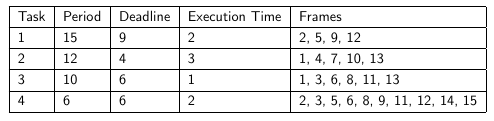
\includegraphics[width=0.7\paperwidth]{./figures/task1_table1.png}
          \caption{A task set and schedule}
        \end{figure}
      \end{itemize}
    \item Is the period P a multiple of the frame f?
      \begin{itemize}
        \item Yes, $15 \cdot f = P$
      \end{itemize}
    \item Is the frame f sufficiently long?
      \begin{itemize}
        \item Yes. We can see this by drawing the schedule or by adding the execution times per frame...
      \end{itemize}
      \begin{figure}
        \centering
        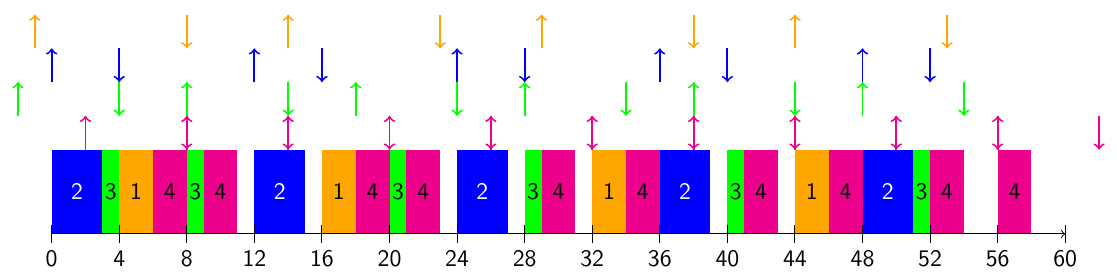
\includegraphics[width=0.7\paperwidth]{./figures/task1_schedule.png}
        \caption{Schedule for Task 1}
      \end{figure}
      \begin{figure}
        \centering
        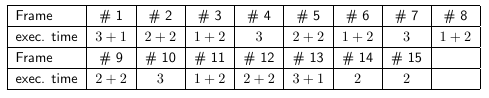
\includegraphics[width=0.7\paperwidth]{./figures/task1_table2.png}
        \caption{Execution time per frame}
      \end{figure}
    \item Determine offsets such that instances start after release time.
      \begin{itemize}
        \item $\Phi_i=\min _{1 \leq j \leq P / T_i}\left\{\left(f_{i, j}-1\right) f-(j-1) T_i\right\}$
        \item $\Phi_1=\min \left\{\begin{array}{l}(2-1) 4-(1-1) 15 \\ (5-1) 4-(2-1) 15 \\ (9-1) 4-(3-1) 15 \\ (12-1) 4-(4-1) 15\end{array} \quad \min \left\{\begin{array}{l}4 \\ 1 \\ 2 \\ -1\end{array}=-1\right.\right.$
        \item $\Phi_2=\min \left\{\begin{array}{l}(1-1) 4-(1-1) 12 \\ (4-1) 4-(2-1) 12 \\ (7-1) 4-(3-1) 12 \\ (10-1) 4-(4-1) 12 \\ (13-1) 4-(5-1) 12\end{array} \quad \min \left\{\begin{array}{l}0 \\ 0 \\ 0 \\ 0 \\ 0\end{array} = 0 \right.\right.$
        \item $\Phi_3=\min \left\{\begin{array}{l}(1-1) 4-(1-1) 10 \\ (3-1) 4-(2-1) 10 \\ (6-1) 4-(3-1) 10 \\ (8-1) 4-(4-1) 10 \\ (11-1) 4-(5-1) 10 \\ (13-1) 4-(6-1) 10\end{array} \quad=\min \left\{\begin{array}{l}0 \\ -2 \\ 0 \\ -2 \\ 0 \\ -2\end{array} = -2 \right.\right.$
        \item $\Phi_4=\min \left\{\begin{array}{l}(2-1) 4-(1-1) 6 \\ (3-1) 4-(2-1) 6 \\ (5-1) 4-(3-1) 6 \\ (6-1) 4-(4-1) 6 \\ (8-1) 4-(5-1) 6 \\ (9-1) 4-(6-1) 6 \\ (11-1) 4-(7-1) 6 \\ (12-1) 4-(8-1) 6 \\ (14-1) 4-(9-1) 6 \\ (15-1) 4-(10-1) 6\end{array} \quad=\min \left\{\begin{array}{l}4 \\ 2 \\ 4 \\ 2 \\ 4 \\ 2 \\ 4 \\ 2 \\ 4 \\ 2\end{array} = 2 \right.\right.$
      \end{itemize}
    \item Are deadlines respected?
      \begin{itemize}
        \item Yes...
        \item $(j-1) T_i+\Phi_i+D_i \geq f_{i, j} f \quad \forall i, 1 \leq j \leq P / T_i$
        \item $\left\{\begin{array}{l}(1-1) 15-1+9=8 \geq 8=2 \cdot 4 \\ (2-1) 15-1+9=23 \geq 20=5 \cdot 4 \\ (3-1) 15-1+9=38 \geq 36=9 \cdot 4 \\ (4-1) 15-1+9=53 \geq 48=12 \cdot 4\end{array}\right.$
        \item $\left\{\begin{array}{l}(1-1) 12+0+4=4 \geq 4=1 \cdot 4 \\ (2-1) 12+0+4=16 \geq 16=4 \cdot 4 \\ (3-1) 12+0+4=28 \geq 28=7 \cdot 4 \\ (4-1) 12+0+4=40 \geq 40=10 \cdot 4 \\ (5-1) 12+0+4=52 \geq 52=13 \cdot 4\end{array}\right.$
        \item $\left\{\begin{array}{l}(1-1) 10-2+6=4 \geq 4=1 \cdot 4 \\ (2-1) 10-2+6=14 \geq 12=3 \cdot 4 \\ (3-1) 10-2+6=24 \geq 24=6 \cdot 4 \\ (4-1) 10-2+6=34 \geq 32=8 \cdot 4 \\ (5-1) 10-2+6=44 \geq 44=11 \cdot 4 \\ (6-1) 10-2+6=54 \geq 52=13 \cdot 4\end{array}\right.$
        \item $\left\{\begin{array}{l}(1-1) 6+2+6=8 \geq 8=2 \cdot 4 \\ (2-1) 6+2+6=14 \geq 12=3 \cdot 4 \\ (3-1) 6+2+6=20 \geq 20=5 \cdot 4 \\ (4-1) 6+2+6=26 \geq 24=6 \cdot 4 \\ (5-1) 6+2+6=32 \geq 32=8 \cdot 4 \\ (6-1) 6+2+6=38 \geq 36=9 \cdot 4 \\ (7-1) 6+2+6=44 \geq 44=11 \cdot 4 \\ (8-1) 6+2+6=50 \geq 48=12 \cdot 4 \\ (9-1) 6+2+6=56 \geq 56=14 \cdot 4 \\ (10-1) 6+2+6=62 \geq 60=15 \cdot 4\end{array}\right.$
      \end{itemize}
  \end{enumerate}
\end{frame}
